\section{Frontend}\label{sec:frontend}
The following section describes our user frontend and especially how we show data to the user in a compact manner.
The frontend is written in Angular using Angular Material library.
We devided the frontend in 5 parts.
The user can choose in a navigation bar between \textit{Dashboard}, \textit{Supplier}, \textit{Consumer}, \textit{Batteries} and \textit{Prices} view.
The views are decribed in the following subsections.

\subsection{Supplier and Consumer}
In the Supplier view the user can create, delete or manage supplier.
Creating, delete or manage consumer works equivalent so we will explain it only for supplier.

\begin{figure}[!h]
    \centering
    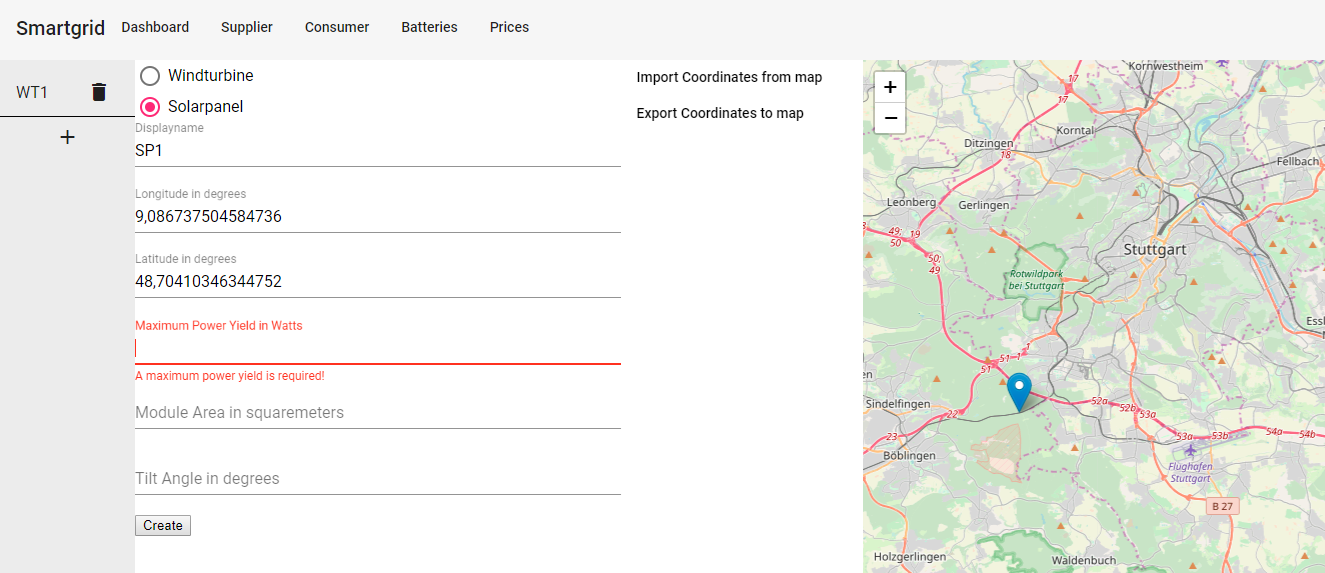
\includegraphics[width=1.00\textwidth]{../figures/supplierView.PNG}
    \caption{View to create, delete or manage suppliers}
    \label{fig:suppliers}
\end{figure}

The interface for suppliers is shown in \cref{fig:suppliers}.
In the left side there is a navigation bar which shows all created supplier.
A user can add a new one using the \textit{plus} button under the suppliers, delete a specific supplier using the \textit{bin} button right to the supplier or manage the supplier clicking on it.
The main part of this page is the form with the user given data such as latitute, longitute or additional supplier specific needed data, e.g. rotator radius for wind turbines.
The kind of supplier can be chosen with the radio button above the form.
Due to angulars modularity it's easy to add more kinds of supplier in the future.
Next to the form is a map using angular leaflet openstreetmap API.
The nice part is that a user does not need to know the specific latitute or longitute to create supplier.
Clicking on the map adds a location point which can be exported easily to the form which allows the user to create suppliers at a specific place in the map.
Once created a supplier, it available in the navigation bar at the right.
Clicking on it shows all data already filled in the form and allows the user to change it during run time.


\subsection{Batteries}
The batteries view is shown in \cref{fig:batteries}.
On the left side of the page there is the same kind of navigation bar we also used in the supplier and consumer pages to create, delete and manage batteries.
In the middle of the view there is also a form to set the batteries data.
The user can specify battery capacity, charge and discharge rates and efficiency as well as it's position.
The position can either set directly through the form or just like in the supplier or consumer view through the map using the export button.

\begin{figure}[!h]
    \centering
    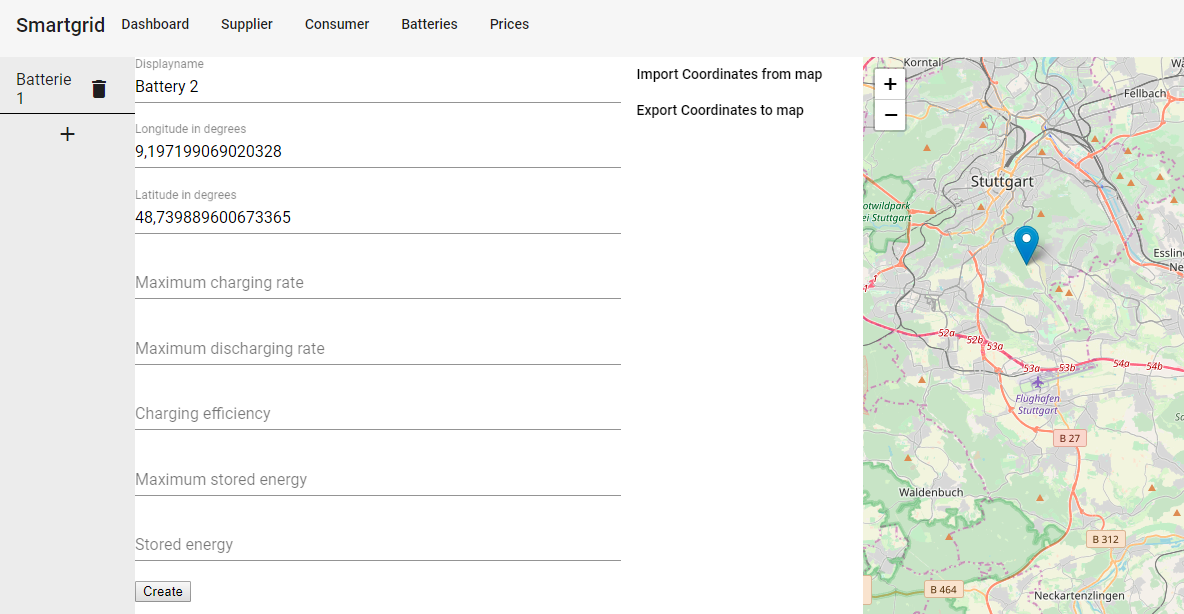
\includegraphics[width=1.00\textwidth]{../figures/batteriesView.PNG}
    \caption{View to create, delete or manage batteries}
    \label{fig:batteries}
\end{figure}


\subsection{Prices}
The prices view shows the energy prices for bidding zone DE-LU as table and bar chart.
The user can specify start and end date of the prices so he can take a look at the day-ahead prices as well as the past 5 days of the energy prices.
The page is shown in \cref{fig:prices}.

\begin{figure}[!h]
    \centering
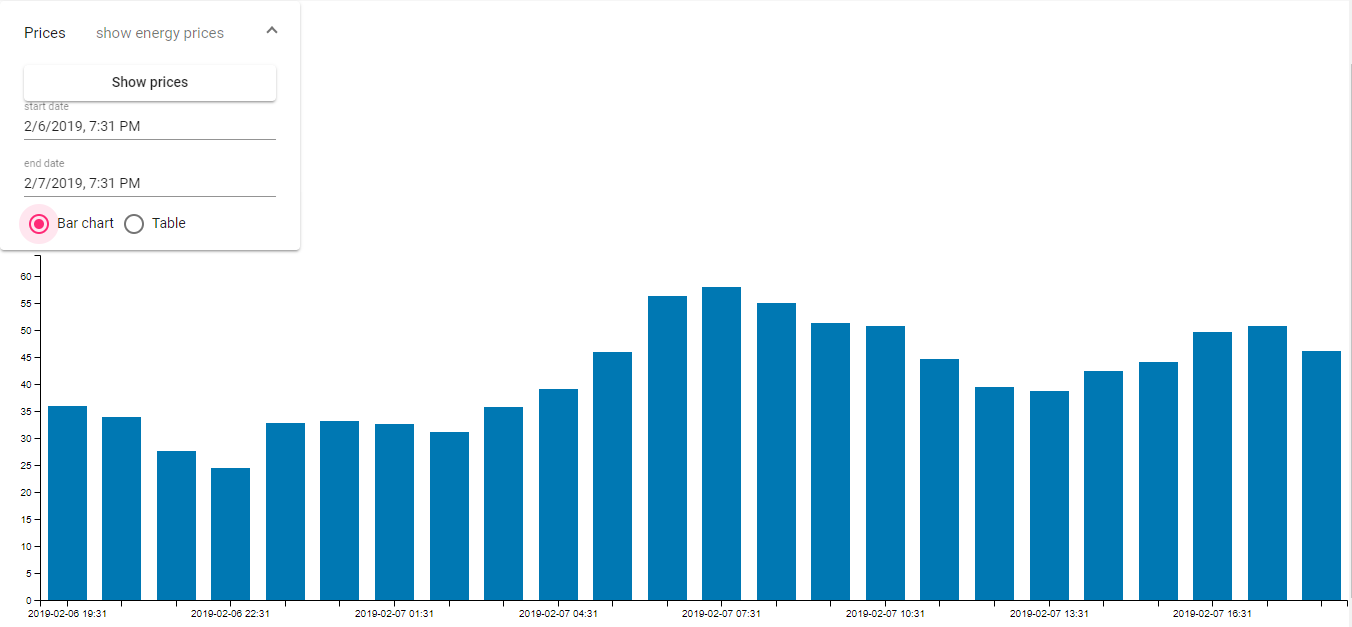
\includegraphics[width=1.00\textwidth]{../figures/prices.PNG}
    \caption{View show energy prices for specific time interval}
    \label{fig:prices}
\end{figure}

\subsection{Dashboard}
The most interesting view is the dashboard.
Here the user can take a look easily at different kinds of information in a compact manner.
The view shows supply, demand and other information in a chart, as shown in \cref{fig:dashboard}

\begin{figure}[!h]
    \centering
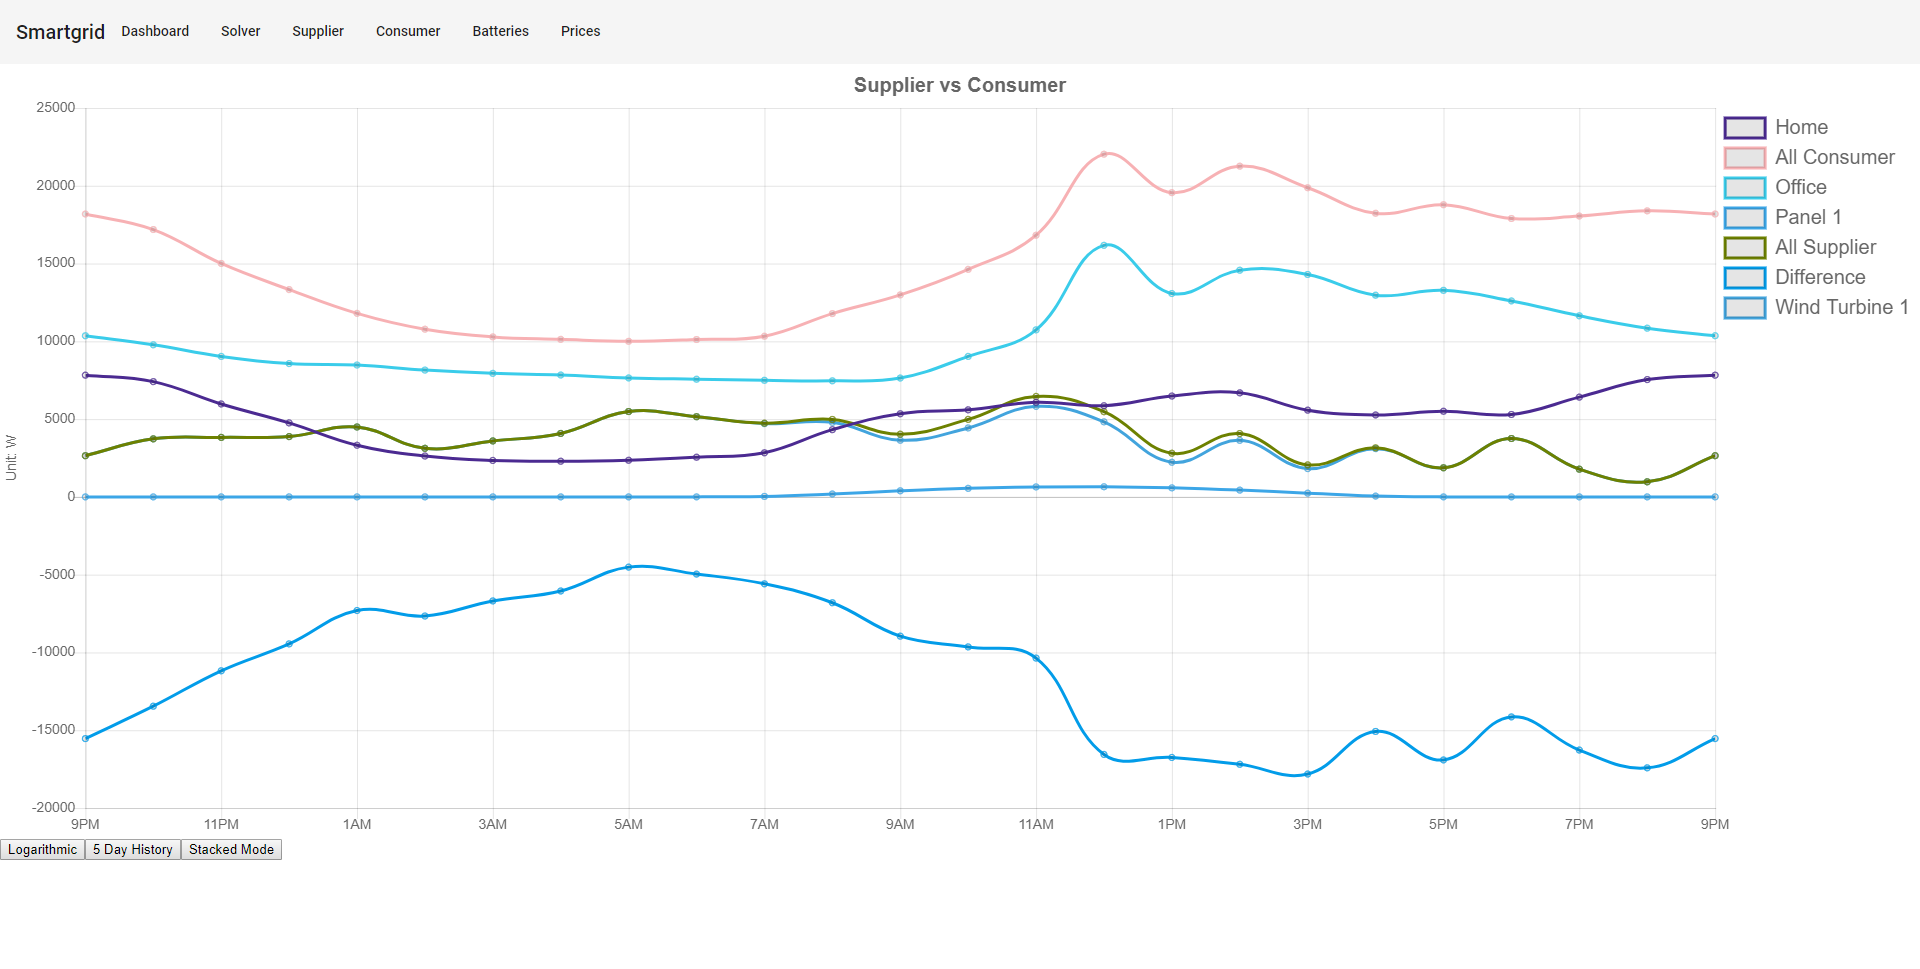
\includegraphics[width=1.00\textwidth]{../figures/Overview.png}
    \caption{Dashboard view to show the charts}
    \label{fig:dashboard}
\end{figure}

Clicking on the data in the legend in the right part of the chart allows the user to disable or enable data in the chart.
This makes the chart more clear and allows the user to concentrate better on the information he is interested in.
\Cref{fig:consumerChart} shows a chart containing only the consumers.

\begin{figure}[!h]
    \centering
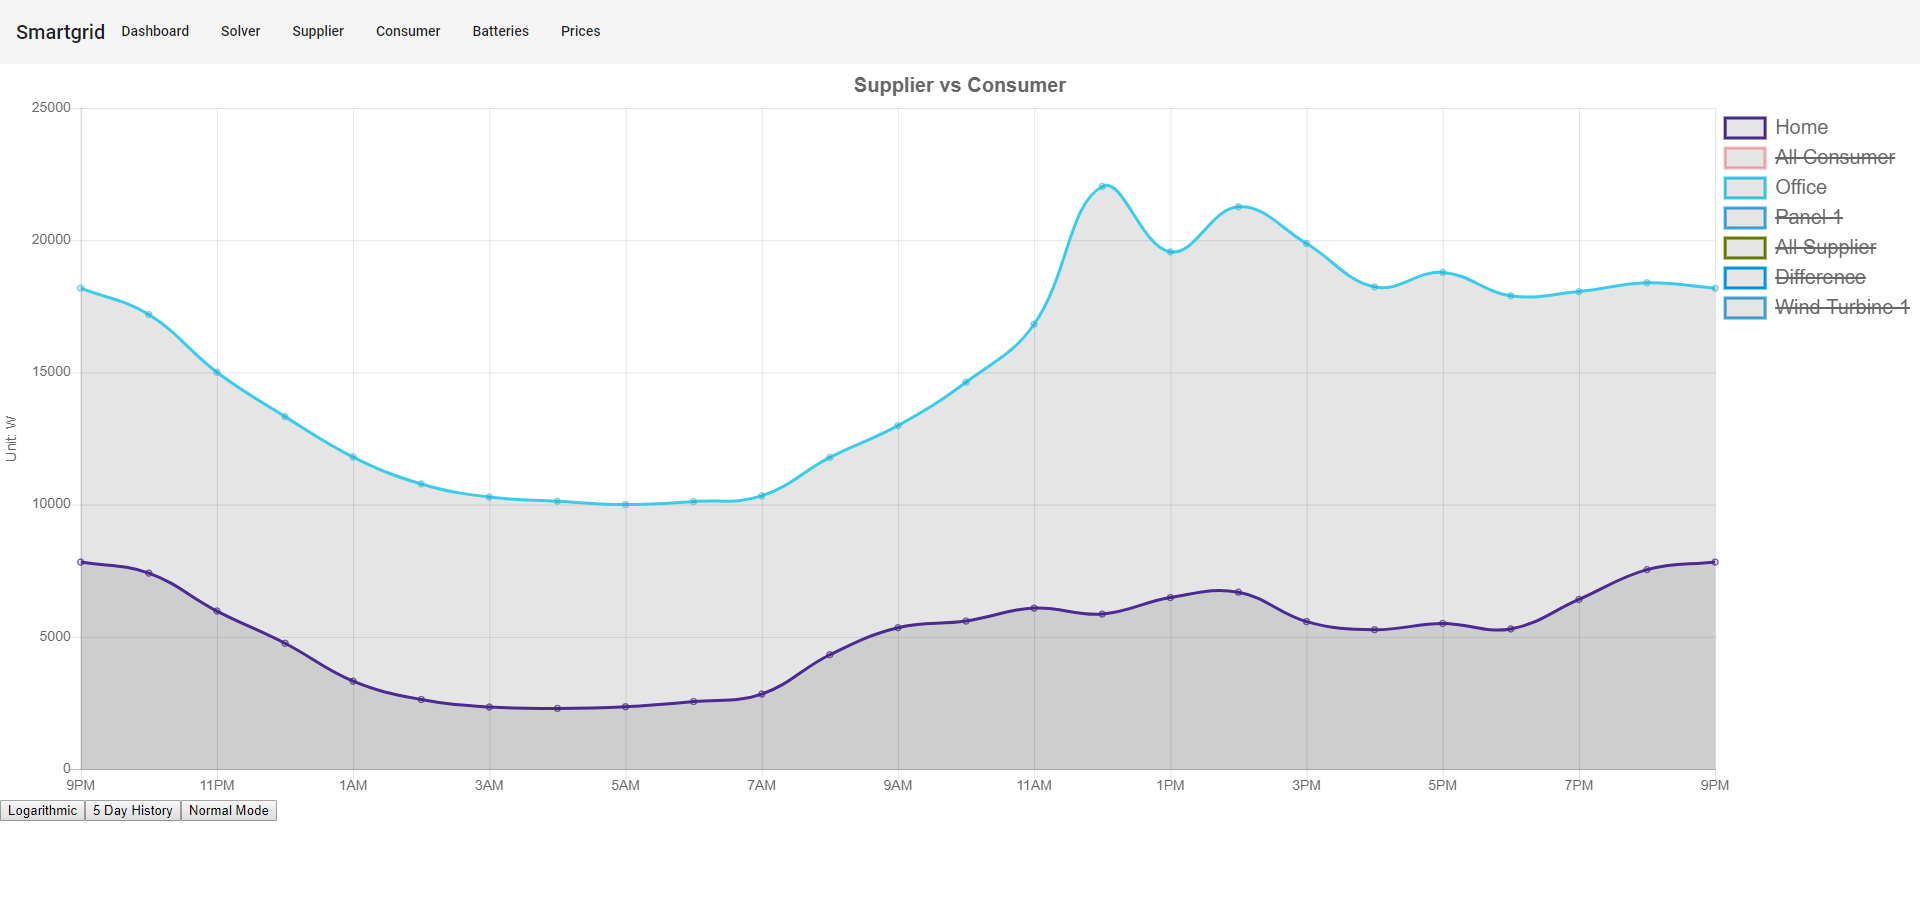
\includegraphics[width=1.00\textwidth]{../figures/ConsumerStacked.png}
    \caption{Chart showing only the energy demand of the consumers}
    \label{fig:consumerChart}
\end{figure}

If a user is interested only in the energy produced by the supplier, he can select only the supplier as shown in \cref{fig:supplierChart}.

\begin{figure}[!h]
    \centering
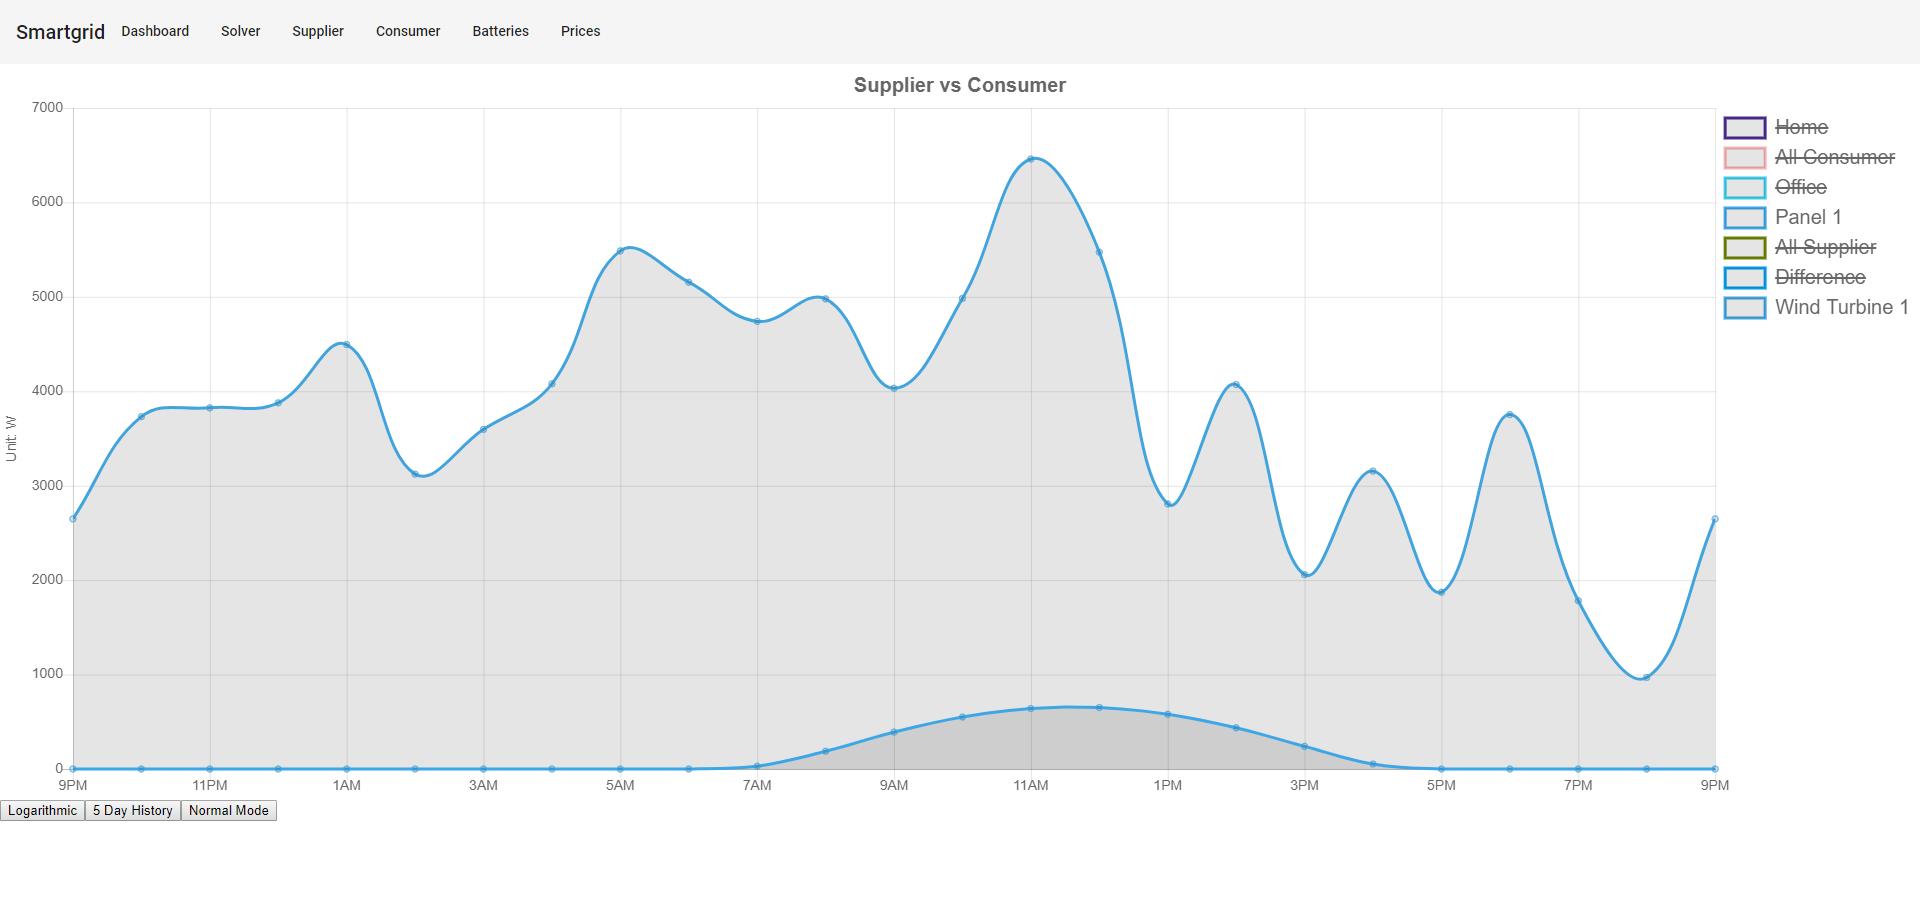
\includegraphics[width=1.00\textwidth]{../figures/SupplierStacked.png}
    \caption{Chart showing only the energy produced by the supplier}
    \label{fig:supplierChart}
\end{figure}

Using the buttons under the chart switches between several charts.
We provide a logarithmic view or normal view.
In addition to this, we can show the user 5 days history or forecast.

For kind of charts we chose to support stacked charts and normal charts.
In stacked charts the values can be stacked above each others.
In  \cref{fig:supplierChart} a stacked chart is used, where the supply of the supplier \textit{Office} added above the supplier \textit{Home}.
\Cref{fig:dashboard} shows a normal chart.